\documentclass[11pt,a4paper]{article}
\usepackage[margin=0.75in]{geometry}
\usepackage{amsmath,amssymb,mathtools}
\usepackage{tikz}
\usetikzlibrary{arrows.meta,calc,patterns,positioning}
\usepackage{enumitem}
\usepackage{booktabs,array,longtable,multicol}
\usepackage{xcolor}
\usepackage{fancyhdr}
\usepackage{tcolorbox}
\tcbuselibrary{breakable,skins}
\usepackage[hidelinks]{hyperref}
\setlength{\parindent}{0pt}
\setlength{\parskip}{4pt}
\setlist[enumerate]{leftmargin=*, itemsep=3pt}
\pagestyle{fancy}
\fancyhf{}
\lhead{BCS-012: Basic Mathematics}
\rhead{December 2024 Solved Paper}
\cfoot{\thepage}
\newcommand{\question}[2]{\begin{tcolorbox}[breakable,colback=gray!5,colframe=black!35,title=\textbf{Question #1}]#2\end{tcolorbox}}
\newcommand{\answer}{\textbf{Solution.}\ }
\newcommand{\R}{\mathbb{R}}
\newcommand{\C}{\mathbb{C}}
\newcommand{\vect}[1]{\overrightarrow{#1}}
\newcommand{\Rs}{Rs.}

\begin{document}
\begin{center}
{\Large\bfseries IGNOU BCS-012: Basic Mathematics}\\[2mm]
{\large\bfseries Term-End Examination, December 2024}\\[1mm]
{\bfseries Full Solved Question Paper with Final Theory Sheet}\\[1mm]
Time: 3 Hours \qquad Maximum Marks: 100
\end{center}

\section*{Solved Paper}

\question{1(a)}{Show that
\[
\begin{vmatrix}
1&a&a^2\\
a^2&1&a\\
a&a^2&1
\end{vmatrix}=(a^3-1)^2 .
\]}
\answer
Expanding along the first row,
\begin{align*}
D&=1\begin{vmatrix}1&a\\ a^2&1\end{vmatrix}
-a\begin{vmatrix}a^2&a\\ a&1\end{vmatrix}
+a^2\begin{vmatrix}a^2&1\\ a&a^2\end{vmatrix}\\
&=(1-a^3)-a(a^2-a^2)+a^2(a^4-a)\\
&=1-a^3+a^6-a^3=a^6-2a^3+1=(a^3-1)^2.
\end{align*}
Hence proved.

\question{1(b)}{If
\[
A=\begin{bmatrix}1&2&2\\2&1&2\\2&2&1\end{bmatrix},
\]
show that $A^2-4A-5I_3=O_3$.}
\answer
First compute
\[
A^2=\begin{bmatrix}1&2&2\\2&1&2\\2&2&1\end{bmatrix}
\begin{bmatrix}1&2&2\\2&1&2\\2&2&1\end{bmatrix}
=\begin{bmatrix}9&8&8\\8&9&8\\8&8&9\end{bmatrix}.
\]
Also,
\[
4A+5I_3=\begin{bmatrix}4&8&8\\8&4&8\\8&8&4\end{bmatrix}
+\begin{bmatrix}5&0&0\\0&5&0\\0&0&5\end{bmatrix}
=\begin{bmatrix}9&8&8\\8&9&8\\8&8&9\end{bmatrix}=A^2.
\]
Therefore $A^2-4A-5I_3=O_3$.

\question{1(c)}{Use the principle of mathematical induction to show that $3^{2n}-1$ is divisible by $8$ for each natural number $n$.}
\answer
Let $P(n)$ be the statement that $3^{2n}-1$ is divisible by $8$.

For $n=1$,
\[
3^{2}-1=9-1=8,
\]
which is divisible by $8$. Thus $P(1)$ is true.

Assume $P(k)$ is true, i.e., $3^{2k}-1=8m$ for some integer $m$. Then
\begin{align*}
3^{2(k+1)}-1&=9\cdot 3^{2k}-1\\
&=9(3^{2k}-1)+8.
\end{align*}
By the induction assumption, $3^{2k}-1$ is divisible by $8$, so $9(3^{2k}-1)+8$ is also divisible by $8$. Hence $P(k+1)$ is true. Therefore, by induction, $3^{2n}-1$ is divisible by $8$ for all $n\in\mathbb N$.

\question{1(d)}{If in an A.P. $a=2$ and the sum of the first five terms is one fourth of the sum of next five terms, show that $a_{20}=-112$.}
\answer
Let the common difference be $d$. The first term is $a=2$.
\[
S_5=\frac{5}{2}[2a+4d]=\frac{5}{2}[4+4d]=10+10d.
\]
The sum of the next five terms is $a_6+a_7+a_8+a_9+a_{10}=S_{10}-S_5$.
\[
S_{10}=\frac{10}{2}[2a+9d]=5[4+9d]=20+45d.
\]
Thus,
\[
S_{10}-S_5=(20+45d)-(10+10d)=10+35d.
\]
Given $S_5=\frac14(S_{10}-S_5)$,
\[
10+10d=\frac14(10+35d).
\]
So,
\[
40+40d=10+35d\quad\Rightarrow\quad 5d=-30\quad\Rightarrow\quad d=-6.
\]
Therefore,
\[
a_{20}=a+19d=2+19(-6)=2-114=-112.
\]
Hence proved.

\question{1(e)}{If $z\in\C$, $|z|=1$, $z\ne -1$, show that
\[
\frac{z-1}{z+1}
\]
is purely imaginary.}
\answer
Since $|z|=1$, we have $z\bar z=1$, hence $\bar z=\frac1z$. Let
\[
w=\frac{z-1}{z+1}.
\]
Then
\begin{align*}
\bar w&=\frac{\bar z-1}{\bar z+1}
=\frac{\frac1z-1}{\frac1z+1}
=\frac{1-z}{1+z}
=-\frac{z-1}{z+1}=-w.
\end{align*}
If $\bar w=-w$, then $w+\bar w=0$, so $\operatorname{Re}(w)=0$. Hence $w$ is purely imaginary.

\question{1(f)}{If two roots $r_1$ and $r_2$ of $x^2+kx+12=0$ are such that $(r_1-r_2)=1$, find $k$.}
\answer
For $x^2+kx+12=0$,
\[
r_1+r_2=-k,\qquad r_1r_2=12.
\]
Given $r_1-r_2=1$. Squaring,
\[
(r_1-r_2)^2=(r_1+r_2)^2-4r_1r_2.
\]
Therefore,
\[
1=(-k)^2-4(12)=k^2-48.
\]
Hence
\[
k^2=49\quad\Rightarrow\quad k=\pm 7.
\]
So the possible values are
\[
\boxed{k=7\text{ or }k=-7.}
\]

\question{1(g)}{Two tailors A and B earn \Rs\ 600 per day and \Rs\ 800 per day respectively. Tailor A can stitch 6 shirts and 4 pants per day, while Tailor B can stitch 10 shirts and 4 pants per day. How many days shall each work if it is desired to produce at least 60 shirts and 32 pants at minimum labour cost? Also calculate the least cost.}
\answer
Let $x$ be the number of days Tailor A works and $y$ be the number of days Tailor B works. We minimize
\[
C=600x+800y
\]
subject to
\[
6x+10y\ge 60,
\qquad 4x+4y\ge 32,
\qquad x\ge0,
\qquad y\ge0.
\]
Equivalently,
\[
3x+5y\ge30,
\qquad x+y\ge8.
\]
The corner points of the feasible region relevant for minimization are:
\[
(10,0),\quad (0,8),\quad \text{and intersection of }3x+5y=30,\ x+y=8.
\]
Solving the intersection:
\[
x+y=8\Rightarrow x=8-y.
\]
Substitute in $3x+5y=30$:
\[
3(8-y)+5y=30\Rightarrow 24+2y=30\Rightarrow y=3,
\]
so $x=5$.

Cost at the corner points:
\[
C(10,0)=6000,
\quad C(0,8)=6400,
\quad C(5,3)=600(5)+800(3)=5400.
\]
Thus the minimum cost is obtained at $(x,y)=(5,3)$.
\[
\boxed{\text{Tailor A should work 5 days and Tailor B should work 3 days.}}
\]
\[
\boxed{\text{Minimum cost}=\Rs\ 5400.}
\]

\begin{center}
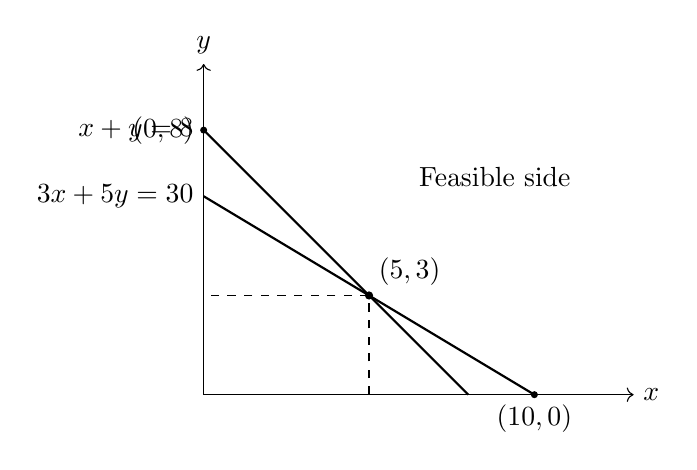
\begin{tikzpicture}[scale=0.42]
\draw[->] (0,0)--(13,0) node[right]{$x$};
\draw[->] (0,0)--(0,10) node[above]{$y$};
\draw[thick] (10,0)--(0,6) node[left]{$3x+5y=30$};
\draw[thick] (8,0)--(0,8) node[left]{$x+y=8$};
\filldraw (5,3) circle (3pt) node[above right]{$(5,3)$};
\filldraw (10,0) circle (2.5pt) node[below]{$(10,0)$};
\filldraw (0,8) circle (2.5pt) node[left]{$(0,8)$};
\draw[dashed] (5,0)--(5,3)--(0,3);
\node at (8.8,6.6) {Feasible side};
\end{tikzpicture}
\end{center}

\question{2(a)}{Using elementary row operations, find inverse of
\[
A=\begin{bmatrix}0&1&2\\1&2&3\\3&1&1\end{bmatrix}.
\]}
\answer
Using row operations on $[A\mid I]$:
\[
\left[\begin{array}{ccc|ccc}
0&1&2&1&0&0\\
1&2&3&0&1&0\\
3&1&1&0&0&1
\end{array}\right]
\sim
\left[\begin{array}{ccc|ccc}
1&0&0&\frac12&-\frac12&\frac12\\
0&1&0&-4&3&-1\\
0&0&1&\frac52&-\frac32&\frac12
\end{array}\right].
\]
Therefore,
\[
\boxed{A^{-1}=\begin{bmatrix}
\frac12&-\frac12&\frac12\\
-4&3&-1\\
\frac52&-\frac32&\frac12
\end{bmatrix}.}
\]

\question{2(b)}{How many terms of the G.P. $\sqrt3,3,3\sqrt3,\ldots$ add up to $39+13\sqrt3$?}
\answer
Here $a=\sqrt3$ and $r=\sqrt3$. The sum of $n$ terms is
\[
S_n=\frac{a(r^n-1)}{r-1}
=\frac{\sqrt3\left((\sqrt3)^n-1\right)}{\sqrt3-1}.
\]
Checking the first six terms:
\[
\sqrt3+3+3\sqrt3+9+9\sqrt3+27=39+13\sqrt3.
\]
Hence,
\[
\boxed{n=6.}
\]

\question{2(c)}{If $1,\omega,\omega^2$ are cube roots of unity, show that
\[
(2+3\omega+2\omega^2)^9(4+3\omega+3\omega^2)^9=1.
\]}
\answer
For cube roots of unity,
\[
1+\omega+\omega^2=0,
\qquad \omega^3=1.
\]
Thus $\omega^2=-1-\omega$. Now,
\begin{align*}
2+3\omega+2\omega^2
&=2+3\omega+2(-1-\omega)=\omega,\\
4+3\omega+3\omega^2
&=4+3\omega+3(-1-\omega)=1.
\end{align*}
Therefore,
\[
(2+3\omega+2\omega^2)^9(4+3\omega+3\omega^2)^9
=\omega^9\cdot 1^9=(\omega^3)^3=1.
\]
Hence proved.

\question{2(d)}{If $\alpha$ and $\beta$ are roots of $3x^2-4x+1=0$, form an equation whose roots are $\dfrac{\alpha^2}{\beta}$ and $\dfrac{\beta^2}{\alpha}$.}
\answer
For $3x^2-4x+1=0$,
\[
\alpha+\beta=\frac43,
\qquad \alpha\beta=\frac13.
\]
Let the new roots be
\[
p=\frac{\alpha^2}{\beta},
\qquad q=\frac{\beta^2}{\alpha}.
\]
Their product is
\[
pq=\frac{\alpha^2\beta^2}{\alpha\beta}=\alpha\beta=\frac13.
\]
Their sum is
\[
p+q=\frac{\alpha^3+\beta^3}{\alpha\beta}.
\]
Now,
\[
\alpha^3+\beta^3=(\alpha+\beta)^3-3\alpha\beta(\alpha+\beta)
=\left(\frac43\right)^3-3\left(\frac13\right)\left(\frac43\right)
=\frac{64}{27}-\frac43=\frac{28}{27}.
\]
Thus,
\[
p+q=\frac{28/27}{1/3}=\frac{28}{9}.
\]
Hence the required equation is
\[
x^2-\frac{28}{9}x+\frac13=0,
\]
or
\[
\boxed{9x^2-28x+3=0.}
\]

\question{3(a)}{Find
\[
\lim_{x\to0}\frac{\sqrt{x+3}-\sqrt3}{x}.
\]}
\answer
Rationalize:
\begin{align*}
\lim_{x\to0}\frac{\sqrt{x+3}-\sqrt3}{x}
&=\lim_{x\to0}\frac{(\sqrt{x+3}-\sqrt3)(\sqrt{x+3}+\sqrt3)}{x(\sqrt{x+3}+\sqrt3)}\\
&=\lim_{x\to0}\frac{x}{x(\sqrt{x+3}+\sqrt3)}\\
&=\frac{1}{2\sqrt3}.
\end{align*}
Therefore,
\[
\boxed{\frac{1}{2\sqrt3}}.
\]

\question{3(b)}{If $y=ae^{mx}+be^{-mx}$, show that
\[
\frac{d^2y}{dx^2}=m^2y.
\]}
\answer
Differentiate once:
\[
\frac{dy}{dx}=am e^{mx}-bm e^{-mx}.
\]
Differentiate again:
\[
\frac{d^2y}{dx^2}=am^2e^{mx}+bm^2e^{-mx}
=m^2(ae^{mx}+be^{-mx})=m^2y.
\]
Hence proved.

\question{3(c)}{Determine the interval in which
\[
f(x)=-2x^3+24x+7
\]
is increasing.}
\answer
A function is increasing where $f'(x)>0$. Here,
\[
f'(x)=-6x^2+24=6(4-x^2).
\]
So
\[
f'(x)>0\iff 4-x^2>0\iff x^2<4\iff -2<x<2.
\]
Therefore, $f(x)$ is increasing on
\[
\boxed{(-2,2).}
\]

\begin{center}
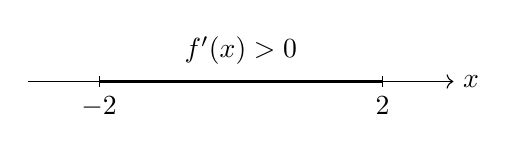
\begin{tikzpicture}[scale=0.9]
\draw[->] (-3,0)--(3,0) node[right]{$x$};
\draw (-2,0.08)--(-2,-0.08) node[below]{$-2$};
\draw (2,0.08)--(2,-0.08) node[below]{$2$};
\draw[very thick] (-2,0)--(2,0);
\node[above] at (0,0.1) {$f'(x)>0$};
\end{tikzpicture}
\end{center}

\question{3(d)}{If a mothball evaporates at a rate proportional to its surface area $4\pi r^2$, show that its radius decreases at a constant rate.}
\answer
The volume of a spherical mothball is
\[
V=\frac{4}{3}\pi r^3.
\]
Since evaporation rate is proportional to surface area and volume decreases,
\[
\frac{dV}{dt}=-k(4\pi r^2),\quad k>0.
\]
Differentiate $V$ with respect to $t$:
\[
\frac{dV}{dt}=4\pi r^2\frac{dr}{dt}.
\]
Therefore,
\[
4\pi r^2\frac{dr}{dt}=-k(4\pi r^2).
\]
For $r\ne0$,
\[
\frac{dr}{dt}=-k.
\]
Thus the radius decreases at the constant rate $k$.

\question{4(a)}{Evaluate
\[
\int \frac{x}{\sqrt{x+3}}\,dx.
\]}
\answer
Put $u=x+3$, so $x=u-3$ and $du=dx$. Then
\begin{align*}
\int \frac{x}{\sqrt{x+3}}\,dx
&=\int \frac{u-3}{\sqrt u}\,du\\
&=\int (u^{1/2}-3u^{-1/2})\,du\\
&=\frac{2}{3}u^{3/2}-6u^{1/2}+C.
\end{align*}
Substituting $u=x+3$,
\[
\boxed{\int \frac{x}{\sqrt{x+3}}\,dx=\frac{2}{3}(x-6)\sqrt{x+3}+C.}
\]

\question{4(b)}{Evaluate
\[
\int_a^b \frac{\log x}{x}\,dx,\qquad a>b>0.
\]}
\answer
Let $u=\log x$. Then $du=\frac{1}{x}dx$. Hence
\[
\int_a^b \frac{\log x}{x}\,dx=\int_{\log a}^{\log b}u\,du
=\frac12\left[(\log b)^2-(\log a)^2\right].
\]
Therefore,
\[
\boxed{\int_a^b \frac{\log x}{x}\,dx=\frac12\left[(\log b)^2-(\log a)^2\right].}
\]

\question{4(c)}{Find the area bounded by $y=\sqrt{x}$ and $y=x$.}
\answer
The curves intersect where
\[
\sqrt{x}=x.
\]
Since $x\ge0$, squaring gives $x=x^2$, so $x=0$ or $x=1$. On $[0,1]$, $\sqrt{x}\ge x$. Therefore, the required area is
\[
A=\int_0^1(\sqrt{x}-x)\,dx
=\left[\frac{2}{3}x^{3/2}-\frac{x^2}{2}\right]_0^1
=\frac23-\frac12=\frac16.
\]
Thus,
\[
\boxed{A=\frac16\text{ square units}.}
\]

\begin{center}
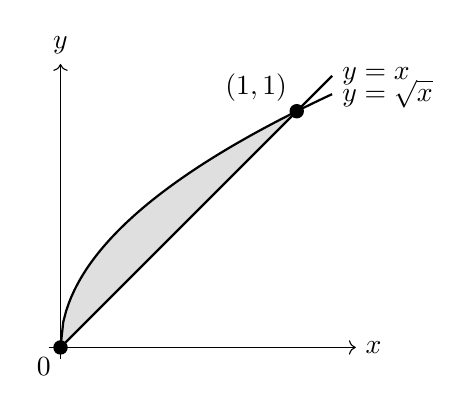
\begin{tikzpicture}[scale=3]
\draw[->] (-0.05,0)--(1.25,0) node[right]{$x$};
\draw[->] (0,-0.05)--(0,1.2) node[above]{$y$};
\fill[gray!25,domain=0:1,samples=100] plot (\x,{sqrt(\x)}) -- plot[domain=1:0] (\x,{\x}) -- cycle;
\draw[thick,domain=0:1.15,samples=100] plot (\x,{sqrt(\x)}) node[right]{$y=\sqrt{x}$};
\draw[thick,domain=0:1.15] plot (\x,{\x}) node[right]{$y=x$};
\filldraw (0,0) circle (0.8pt) node[below left]{$0$};
\filldraw (1,1) circle (0.8pt) node[above left]{$(1,1)$};
\end{tikzpicture}
\end{center}

\question{4(d)}{If $\vec a$ and $\vec b$ are two vectors, show that
\[
|\vec a+\vec b|\le |\vec a|+|\vec b|.
\]}
\answer
This is the triangle inequality. We prove it using dot product:
\begin{align*}
|\vec a+\vec b|^2
&=(\vec a+\vec b)\cdot(\vec a+\vec b)\\
&=|\vec a|^2+2\vec a\cdot\vec b+|\vec b|^2.
\end{align*}
Since $\vec a\cdot\vec b\le |\vec a|\,|\vec b|$,
\[
|\vec a+\vec b|^2\le |\vec a|^2+2|\vec a|\,|\vec b|+|\vec b|^2
=(|\vec a|+|\vec b|)^2.
\]
Taking square roots,
\[
\boxed{|\vec a+\vec b|\le |\vec a|+|\vec b|.}
\]

\question{5(a)}{Show that the lines
\[
\frac{x-5}{4}=\frac{y-7}{4}=\frac{z+3}{-5}
\]
and
\[
\frac{x-8}{7}=\frac{y-4}{1}=\frac{z-5}{3}
\]
intersect.}
\answer
Write the first line as
\[
x=5+4t,
\quad y=7+4t,
\quad z=-3-5t.
\]
Write the second line as
\[
x=8+7s,
\quad y=4+s,
\quad z=5+3s.
\]
For intersection, solve
\[
5+4t=8+7s,
\quad 7+4t=4+s,
\quad -3-5t=5+3s.
\]
The solution is
\[
t=-1,
\qquad s=-1.
\]
Substituting in the first line,
\[
x=5+4(-1)=1,
\quad y=7+4(-1)=3,
\quad z=-3-5(-1)=2.
\]
Substituting in the second line gives the same point:
\[
x=8+7(-1)=1,
\quad y=4+(-1)=3,
\quad z=5+3(-1)=2.
\]
Thus the lines intersect at
\[
\boxed{(1,3,2).}
\]

\question{5(b)}{Solve the inequality
\[
\left|\frac{x-3}{2}\right|\le1.
\]}
\answer
\[
\left|\frac{x-3}{2}\right|\le1
\iff -1\le\frac{x-3}{2}\le1.
\]
Multiplying by $2$,
\[
-2\le x-3\le2.
\]
Adding $3$,
\[
1\le x\le5.
\]
Therefore,
\[
\boxed{x\in[1,5].}
\]

\begin{center}
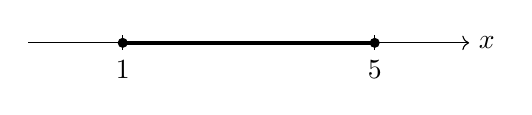
\begin{tikzpicture}[scale=0.8]
\draw[->] (-0.5,0)--(6.5,0) node[right]{$x$};
\foreach \x in {1,5}{\draw (\x,0.12)--(\x,-0.12) node[below]{\x};}
\draw[very thick] (1,0)--(5,0);
\filldraw (1,0) circle (2pt);
\filldraw (5,0) circle (2pt);
\end{tikzpicture}
\end{center}

\question{5(c)}{Using determinants, find the area of a triangle whose vertices are $(1,2)$, $(-2,3)$ and $(-3,-4)$.}
\answer
The area of a triangle with vertices $(x_1,y_1)$, $(x_2,y_2)$ and $(x_3,y_3)$ is
\[
\Delta=\frac12\left|
\begin{vmatrix}
x_1&y_1&1\\
x_2&y_2&1\\
x_3&y_3&1
\end{vmatrix}
\right|.
\]
Thus,
\begin{align*}
\Delta&=\frac12\left|
\begin{vmatrix}
1&2&1\\
-2&3&1\\
-3&-4&1
\end{vmatrix}
\right|\\
&=\frac12|1(3+4)-2(-2+3)+1(8+9)|\\
&=\frac12|7-2+17|=\frac12(22)=11.
\end{align*}
Therefore,
\[
\boxed{\text{Area}=11\text{ square units}.}
\]

\question{5(d)}{If
\[
y=\log_e\left[e^x\left(\frac{x-2}{x+2}\right)^{3/4}\right],
\]
find $\dfrac{dy}{dx}$.}
\answer
Using logarithmic properties,
\[
y=\log_e(e^x)+\log_e\left[\left(\frac{x-2}{x+2}\right)^{3/4}\right]
=x+\frac34\log_e\left(\frac{x-2}{x+2}\right).
\]
So,
\begin{align*}
\frac{dy}{dx}
&=1+\frac34\left(\frac{1}{x-2}-\frac{1}{x+2}\right)\\
&=1+\frac34\left(\frac{4}{x^2-4}\right)\\
&=1+\frac{3}{x^2-4}.
\end{align*}
Therefore,
\[
\boxed{\frac{dy}{dx}=1+\frac{3}{x^2-4}.}
\]

\newpage
\section*{Theory and Formula Sheet for This Paper}

\begin{tcolorbox}[breakable,colback=blue!3,colframe=blue!40,title=\textbf{Important theory, formulas and methods}]
\begin{multicols}{2}
\textbf{Determinants}
\[
\begin{vmatrix}a&b\\c&d\end{vmatrix}=ad-bc.
\]
For a $3\times3$ determinant, expand along a convenient row or column. Row/column operations may simplify the determinant.

\textbf{Matrix inverse}
To find $A^{-1}$ using elementary row operations:
\[
[A\mid I]\to[I\mid A^{-1}].
\]
If $A^2-4A-5I=O$, then $A^2=4A+5I$.

\textbf{Mathematical induction}
To prove $P(n)$ for all $n\in\mathbb N$:
\begin{enumerate}
\item Prove $P(1)$.
\item Assume $P(k)$.
\item Prove $P(k+1)$.
\end{enumerate}

\textbf{A.P.}
\[
a_n=a+(n-1)d,
\qquad S_n=\frac n2[2a+(n-1)d].
\]

\textbf{G.P.}
\[
S_n=\frac{a(r^n-1)}{r-1}\quad(r\ne1).
\]

\textbf{Quadratic roots}
For $ax^2+bx+c=0$:
\[
\alpha+\beta=-\frac ba,
\qquad \alpha\beta=\frac ca.
\]
Also,
\[
(\alpha-\beta)^2=(\alpha+\beta)^2-4\alpha\beta.
\]

\textbf{Complex numbers}
If $|z|=1$, then
\[
z\bar z=1,
\qquad \bar z=\frac1z.
\]
A number $w$ is purely imaginary if
\[
\bar w=-w.
\]

\textbf{Cube roots of unity}
\[
1+\omega+\omega^2=0,
\qquad \omega^3=1.
\]

\textbf{Limits}
Rationalize expressions containing square roots:
\[
\frac{\sqrt{x+a}-\sqrt a}{x}
=\frac{1}{\sqrt{x+a}+\sqrt a}.
\]

\textbf{Differentiation}
\[
\frac{d}{dx}e^{mx}=me^{mx},
\qquad
\frac{d}{dx}e^{-mx}=-me^{-mx}.
\]
A function is increasing where $f'(x)>0$.

\textbf{Sphere}
\[
V=\frac43\pi r^3,
\qquad S=4\pi r^2.
\]
If $\frac{dV}{dt}$ is proportional to $S$, then $\frac{dr}{dt}$ becomes constant.

\textbf{Integration}
\[
\int x^n dx=\frac{x^{n+1}}{n+1}+C\quad(n\ne -1).
\]
\[
\int \frac{\log x}{x}dx=\frac12(\log x)^2+C.
\]

\textbf{Area between curves}
If upper curve is $y=f(x)$ and lower curve is $y=g(x)$,
\[
A=\int_a^b[f(x)-g(x)]dx.
\]

\textbf{Vectors}
\[
\vec a\cdot\vec b=|\vec a|\,|\vec b|\cos\theta.
\]
Triangle inequality:
\[
|\vec a+\vec b|\le |\vec a|+|\vec b|.
\]

\textbf{Line in 3D}
\[
\frac{x-x_1}{l}=\frac{y-y_1}{m}=\frac{z-z_1}{n}=t.
\]
To check intersection of two lines, write both in parametric form and solve for the parameters.

\textbf{Inequality with modulus}
\[
|X|\le a\iff -a\le X\le a\quad(a\ge0).
\]

\textbf{Area of triangle by determinant}
\[
\Delta=\frac12\left|
\begin{vmatrix}
x_1&y_1&1\\
x_2&y_2&1\\
x_3&y_3&1
\end{vmatrix}\right|.
\]

\textbf{Linear programming}
Write variables, objective function, constraints, feasible region, corner points, and then evaluate the objective function at each corner point.
\end{multicols}
\end{tcolorbox}

\end{document}
